\section{Direction-Aware $\lambda$: A Natural Fix That Fails Architecturally}
\label{sec:direction-aware}

Section~\ref{sec:rq2rq3}'s trade-off suggests an obvious refinement: regularize only the codes that need it, decoupling the regularizer's strength per target modality ($\lambda_{\text{img}}$/$\lambda_{\text{txt}}$) instead of one shared $\lambda$ (a per-row loss weight, unit-tested to reduce to the existing single-$\lambda$ path when $\lambda_{\text{img}}=\lambda_{\text{txt}}$). We test three settings: \textbf{img3txt0} ($\lambda_{\text{img}}=3.0$, $\lambda_{\text{txt}}=0.0$), \textbf{img3txt0p3} ($\lambda_{\text{img}}=3.0$, $\lambda_{\text{txt}}=0.3$), and \textbf{img0txt3} ($\lambda_{\text{img}}=0.0$, $\lambda_{\text{txt}}=3.0$) -- the mirror-image cell, regularizing \emph{only} the text side, which directly tests whether text-side pressure alone is sufficient to cause the I$\to$T collapse.

\begin{table}[t]
\centering
\caption{Direction-aware $\lambda$ vs.\ the uniform baselines, MSCOCO T$\to$I / I$\to$T Recall@1, mean $\pm$ std across seeds.}
\label{tab:direction-aware}
\footnotesize
\begin{tabular}{@{}lrrrr@{}}
\toprule
Variant & $\lambda_{\text{img}}$ & $\lambda_{\text{txt}}$ & T$\to$I R@1 & I$\to$T R@1 \\
\midrule
vanilla      & 0.0 & 0.0 & 20.78 $\pm$ 0.06\% & \textbf{10.30 $\pm$ 0.67\%} \\
strong       & 3.0 & 3.0 & \textbf{23.33 $\pm$ 0.11\%} & 0.03 $\pm$ 0.02\% \\
img3txt0     & 3.0 & 0.0 & 7.87 $\pm$ 0.12\% & 0.12 $\pm$ 0.04\% \\
img3txt0p3   & 3.0 & 0.3 & 5.56 $\pm$ 0.13\% & 0.13 $\pm$ 0.05\% \\
img0txt3     & 0.0 & 3.0 & 6.53 $\pm$ 0.08\% & 0.03 $\pm$ 0.01\% \\
\bottomrule
\end{tabular}
\\[2pt]
\footnotesize vanilla/strong: 5 seeds (Table~\ref{tab:table2}). img3txt0/img3txt0p3/img0txt3: 3 seeds each -- img3txt0/img3txt0p3 originally failed 12/12 decode attempts (fp16 nondeterminism on concentrated codebooks, Section~\ref{sec:limitations}); a robustness fix resolved it, and all seeds shown completed via valid beam search (img0txt3 hit no such dead-end).
\end{table}

\paragraph{The hypothesis fails on all three counts.} No setting recovers I$\to$T: all three stay collapsed, 3-seed means ($0.12\pm0.04\%$/$0.13\pm0.05\%$/$0.03\pm0.01\%$) -- true even for img3txt0 and img0txt3, each with one loss weight at exactly zero. img0txt3's I$\to$T ($0.03\pm0.01\%$) is numerically indistinguishable from strong's full-regularization collapse ($0.03\pm0.02\%$, no test run given both are thin samples): text-side pressure \emph{alone} collapses I$\to$T as completely as regularizing both sides, the cleanest evidence text-side regularization suffices on its own. T$\to$I is \emph{worse than vanilla} in all three cells ($7.87\%$/$5.56\%$/$6.53\%$ vs.\ $20.78\%$), not merely worse than strong: every asymmetric setting underperforms both baselines, regardless of which side carries the weight.

\begin{figure}[t]
\centering
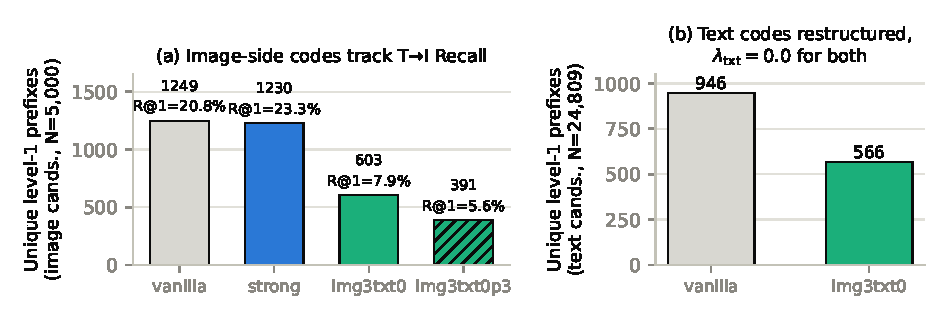
\includegraphics[width=0.92\textwidth]{figures/fig_prefixes.pdf}
\caption{Unique level-1 RQ prefixes by variant -- level-1 is the first token of the semantic ID, the level constrained beam search prunes on first. (a) Image-side count tracks T$\to$I Recall (3-seed mean) almost monotonically. (b) Text-side prefixes, vanilla vs.\ img3txt0 -- both have $\lambda_{\text{txt}}=0.0$, yet img3txt0's text codes are visibly restructured: direct evidence that image-side regularization reaches text-side structure through the shared encoder and codebook.}
\label{fig:prefixes}
\end{figure}

\paragraph{Mechanism: the codebook is not decomposable per modality.} Not an implementation bug: the per-row weight is applied correctly (a shape assertion never fired across training; img3txt0's training loss lands almost exactly half of strong's, as expected if half the rows carry $\lambda=3$ and half carry $\lambda=0$). Zero text-side weight does not protect text-side structure: image and text rows share one encoder forward pass, the same contrastive/reconstruction losses, and one EMA-updated codebook at every level. Figure~\ref{fig:prefixes}(b) shows this directly: under img3txt0, text candidates' codes are measurably restructured relative to vanilla ($566$ vs.\ $946$ unique level-1 prefixes) despite exactly zero text-side loss weight. This also explains the T$\to$I ordering in Figure~\ref{fig:prefixes}(a): unique image-side level-1 codes track T$\to$I Recall almost monotonically -- strong preserves level-1 diversity while flattening mid-levels into constants the decoder learns easily; the asymmetric settings instead concentrate level-1 itself, with no such payoff. Overall, the natural fix is dominated by both uniform-$\lambda$ alternatives on every metric measured -- not because the right combination remains to be tuned, but because a shared encoder and codebook give a per-row loss weight no mechanism to produce a per-modality effect.

\paragraph{Tokenizer-level corroboration.} All three asymmetric variants are Stage-1 checkpoints with no Stage-2 seed involved, so the same decoder-free probe that localized the main I$\to$T collapse (Table~\ref{tab:localization}) runs on them directly. All three collapse on I$\to$T at the tokenizer level ($0.02\%$/$0.02\%$/$0.02\%$ dense R@1, matching weak/medium/strong's $\leq0.04\%$ band, far below vanilla's $7.52\%$), numerically indistinguishable from strong's despite img0txt3's zero image-side weight. The probe also reproduces T$\to$I-worse-than-vanilla for all three ($14.13\%$/$11.81\%$/$8.67\%$ vs.\ vanilla's $26.65\%$); img0txt3's relative ordering differs slightly between dense and decoder-level (worst vs.\ middle), a minor discrepancy noted rather than papered over -- the collapse and worse-than-both-baselines pattern hold regardless. Tokenizer- and decoder-level evidence otherwise agree independently.
